\documentclass[10pt]{jsarticle}
\usepackage[margin=15truemm]{geometry}
\usepackage[dvipdfmx]{graphicx}
\usepackage{ascmac} % for screen
\usepackage{subfigure} % for subfigure
\usepackage{multicol}
\usepackage{amsmath}
\usepackage{mathtools}
\usepackage{amssymb}
\usepackage{multicol}
\usepackage{tikz}
\usetikzlibrary{intersections, calc, arrows.meta}
\usepackage{wrapfig}
\usepackage{setspace} 


\begin{document}
\section{計算}
\begin{itembox}[l]{分配法則}
	\begin{Large}
		\begin{itemize}
			\item $(3x+4y)-(x+y)=$
			\item $2(3x+2y)-3(4x-3y)=$
			\item $(4ab^2-3a-7)-(-7+5a-3ab^2)=$
			\item $\frac{x-y}{3}-\frac{x-2y}{2}=$
		\end{itemize}
	\end{Large}
\end{itembox}

\subsection{文字の利用}
\begin{itembox}[l]{[?]について解く}
	\begin{Large}
		\begin{itemize}
			\item $x+y=2 \quad[x]$\\
			\item $V=\frac{1}{3}sh \quad[h]$\\
			\item $b=\frac{2a+3}{5} \quad[a]$\\
			\item $t=3(a+b+c) \quad[a]$\\
		\end{itemize}
	\end{Large}
\end{itembox}


\subsection{連立方程式}
\begin{itembox}[l]{}
	\begin{Large}
		\begin{itemize}
			\item $
				      \left\{
				      \begin{array}{l}
					      3x-y=13 \\
					      2x+3y=5
				      \end{array}
				      \right.
			      $\\\\
			\item $
				      \left\{
				      \begin{array}{l}
					      2x+y=-3 \\
					      x=3y+2
				      \end{array}
				      \right.
			      $\\\\
			\item $
				      \left\{
				      \begin{array}{l}
					      3x+4y=6 \\
					      \frac{1}{4}x-\frac{1}{3}y=1
				      \end{array}
				      \right.
			      $\\\\
		\end{itemize}
	\end{Large}
\end{itembox}


\section{関数}
\subsection{関数の一般式}
\begin{itembox}[l]{一般式をかけ}
	\begin{multicols}{3}
		\begin{itemize}
			\item 一次関数
			\item 比例
			\item 反比例
		\end{itemize}
	\end{multicols}
\end{itembox}

\subsection{一次関数}
\begin{itembox}[l]{一般式の定数を説明せよ}
	\begin{multicols}{3}
		\begin{itemize}
			\item 傾き
			\item 切片
			\item 変化の割合
		\end{itemize}
	\end{multicols}
\end{itembox}

\begin{itembox}[l]{一般式を求めよ}
	\begin{itemize}
		\item 傾きが3で$(-2,-3)$を通る\\
		\item 変化の割合が2で$x=-1のときy=4$\\\\
		\item $(1,3)と(3,11)$を通る\\\\
		\item $x=−1のときy=−11で、x=4のときy=4$\\\\
		\item $y=-2x+5$に平行で$(4,5)$を通る\\\\
	\end{itemize}
\end{itembox}

\begin{itembox}[l]{次の2直線の交点を求めよ}
	\begin{itemize}
		\item $y=x+3, y=2x-4$\\\\
		      \item$ x+3y=2, 2x+y=-3$\\\\
	\end{itemize}
\end{itembox}




\begin{itembox}[l]{入試に使えるテクニック}
	\begin{itemize}
		\item 2点$(x_1,y_1),(x_2,y_2)$の中点\\
		\item 2点の傾きのみをもとめる(式は求めなくても良い)\\
		\item 三角形の一つの頂点を通り面積を二等分\\
		\item 平行四辺形や長方形の面積を二等分\\
	\end{itemize}
\end{itembox}

\subsection{グラフの問題}

\begin{itembox}[l]{}
	$グラフのような\triangle OABの面積を求めなさい、また点Bを通り\triangle OABを二等分するような直線を求めろ$

	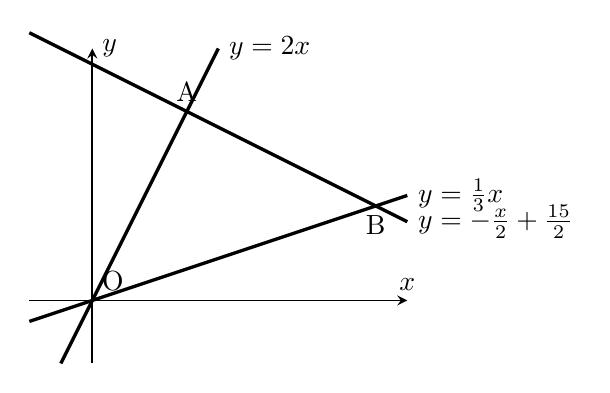
\begin{tikzpicture}[scale=0.4]
		\draw[->,>=stealth,semithick] (-2,0)--(10,0)node[above]{$x$}; %x軸
		\draw[->,>=stealth,semithick] (0,-2)--(0,8)node[right]{$y$}; %y軸
		\draw (0,0)node[above right]{O}; %原点
		\coordinate[label=above:A](P)at(3,6);
		\coordinate[label=below:B](Q)at(9,3);
		\draw[very thick,domain=-1:4] plot(\x, {2*\x})node[right]{$y=2x$};
		\draw[very thick,domain=-2:10] plot(\x, {\x/3})node[right]{$y=\frac{1}{3}x$};
		\draw[very thick,domain=-2:10] plot(\x, {-\x/2+15/2})node[right]{$y=-\frac{x}{2}+\frac{15}{2}$};
	\end{tikzpicture}
\end{itembox}

\begin{itembox}[l]{}
	$A(0,1), B(3,1), C(2,6)のとき、平行四辺形ABDCとなるような点Dの座標を求めよ、また平行四辺形の面積を二等分するような原点をとおる直線を求めろ$

	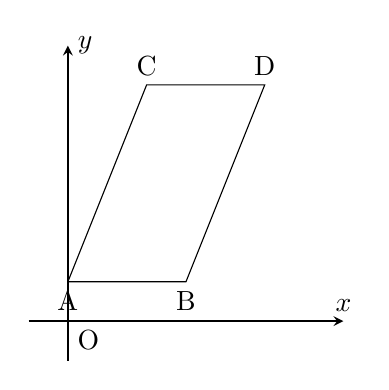
\begin{tikzpicture}[scale=0.5]
		\draw[->,>=stealth,semithick] (-1,0)--(7,0)node[above]{$x$}; %x軸
		\draw[->,>=stealth,semithick] (0,-1)--(0,7)node[right]{$y$}; %y軸
		\draw (0,0)node[below right]{O}; %原点
		\coordinate[label=below:A](P)at(0,1);
		\coordinate[label=below:B](Q)at(3,1);
		\coordinate[label=above:C](R)at(2,6);
		\coordinate[label=above:D](S)at(5,6);
		\draw(P)--(Q)--(S)--(R)--(P);
	\end{tikzpicture}
\end{itembox}





\begin{itembox}[l]{四角形OACBの面積と同じ大きさとなる三角形OADをx軸上にを求めろ。$A(0,6),B(9,0),C(5,5)$}
	\begin{tikzpicture}[scale=0.3]
		\draw[->,>=stealth,semithick] (-1,0)--(14,0)node[above]{$x$}; %x軸
		\draw[->,>=stealth,semithick] (0,-1)--(0,8)node[right]{$y$}; %y軸
		\draw (0,0)node[below right]{O}; %原点
		\draw (0,6)node[left]{$A$}; %点(-1,0)
		\draw (9,0)node[below]{$B$}; %点(0,1)
		\draw (5,5)node[above]{$C$};
		\draw(0,6)--(5,5)--(9,0);
	\end{tikzpicture}
\end{itembox}
\newpage

\section{図形}
\subsection{角度}
\begin{itembox}[l]{次の角を説明せよ}
	\begin{itemize}
		\item  対頂角
		\item 同位角
		\item 錯角
	\end{itemize}
\end{itembox}

\subsection{内角,外角}
\begin{itembox}[l]{次の図形の内角と外角の値を答えよ}
	\begin{itemize}
		\item  三角形
		\item 四角形
		\item n角形
	\end{itemize}
\end{itembox}

\subsection{合同}
\begin{itembox}[l]{三角形の合同条件}
	\begin{Large}
		\begin{itemize}
			\item
			\item
			\item
		\end{itemize}
	\end{Large}
\end{itembox}

\begin{itembox}[l]{証明の基本の書き方}
	. \\[70mm]
\end{itembox}


\begin{itembox}[l]{直角三角形の合同条件}
	\begin{Large}
		\begin{itemize}
			\item
			\item
		\end{itemize}
	\end{Large}
\end{itembox}

\subsection{図形の性質}
\begin{itembox}[l]{二等辺三角形の性質}
	\begin{Large}
		\begin{itemize}
			\item
			\item
			\item
		\end{itemize}
	\end{Large}
\end{itembox}

\begin{itembox}[l]{平行四辺形の定義}
	\begin{Large}
		\begin{itemize}
			\item
		\end{itemize}
	\end{Large}
\end{itembox}

\begin{itembox}[l]{平行四辺形の性質}
	\begin{Large}
		\begin{itemize}
			\item
			\item
			\item
		\end{itemize}
	\end{Large}
\end{itembox}

\begin{itembox}[l]{平行四辺形になる条件}
	\begin{Large}
		\begin{itemize}
			\item
			\item
			\item
			\item
			\item
		\end{itemize}
	\end{Large}
\end{itembox}

\begin{itembox}[l]{長方形の性質}
	\begin{Large}
		\begin{itemize}
			\item
			\item
		\end{itemize}
	\end{Large}
\end{itembox}

\begin{itembox}[l]{ひし形の性質}
	\begin{Large}
		\begin{itemize}
			\item
			\item
		\end{itemize}
	\end{Large}
\end{itembox}

\begin{itembox}[l]{正方形の性質}
	\begin{Large}
		\begin{itemize}
			\item
			\item
			\item
			\item
		\end{itemize}
	\end{Large}
\end{itembox}

\newpage

\section{場合の数,確率}
\begin{itembox}[l]{次の場合の分母を求めよ}
	\begin{multicols}{2}
		\begin{itemize}
			\item サイコロ2つ\vspace{5mm}
			\item サイコロ3つ\vspace{5mm}
			\item コイン2枚\vspace{5mm}
			\item コイン3枚\vspace{5mm}
			\item 5人から2人選出する\vspace{5mm}
			\item 5人から2人並べる\vspace{5mm}
			\item 1,2,3,4の数字から2桁の整数\vspace{5mm}
			\item 0,1,2,3,4の数字から2桁の整数\vspace{5mm}
		\end{itemize}
	\end{multicols}

\end{itembox}
\begin{itembox}[l]{倍数判定法}
	\begin{multicols}{2}
		\begin{itemize}
			\item 偶数,奇数\vspace{5mm}
			\item 3の倍数\vspace{5mm}
			\item 4の倍数\vspace{5mm}
			\item 9の倍数
		\end{itemize}
	\end{multicols}
\end{itembox}

\begin{itembox}[l]{サイコロ2つ}
	\begin{multicols}{2}
		\begin{itemize}
			\item 和が3の倍数\vspace{5mm}
			\item 積が偶数\vspace{5mm}
			\item 積が12の約数\vspace{5mm}
		\end{itemize}
	\end{multicols}
\end{itembox}

\begin{itembox}[l]{コイン3枚}
	\begin{multicols}{2}
		\begin{itemize}
			\item 全て表\vspace{5mm}
			\item 少なくとも1枚表\vspace{5mm}
		\end{itemize}
	\end{multicols}
\end{itembox}

\section{データ}
\begin{itembox}[l]{次の用語を説明せよ}
	\begin{multicols}{2}
		\begin{itemize}
			\item 中央値\vspace{5mm}
			\item 第1四分位数\vspace{5mm}
			\item 第2四分位数\vspace{5mm}
			\item 第3四分位数\vspace{5mm}
			\item 範囲\vspace{5mm}
			\item 四分位範囲\vspace{5mm}
		\end{itemize}
	\end{multicols}
\end{itembox}
\begin{itembox}[l]{箱ひげ図}
	\vspace{30mm}
\end{itembox}
\begin{itembox}[l]{平均、各値がわからない時}
	\vspace{2cm}
\end{itembox}





\end{document}
